\documentclass{article}

\usepackage[utf8]{inputenc}
\usepackage[T1]{fontenc}
\usepackage[english]{babel}
\usepackage{graphicx}
\usepackage{float}
\usepackage[colorlinks=true,linkcolor=black,citecolor=black,urlcolor=blue]{hyperref}
\usepackage[backend=biber]{biblatex}
\addbibresource{references.bib}

% \usepackage[superscript,nomove]{cite}
% \renewcommand{\citeleft}{}
% \renewcommand{\citeright}{}

\title{Slavic Text Restoration}
\author{Maxim Eremeev \and Oleksandr Sychov}
\date{}

\begin{document}

\maketitle

\section{Introduction}
\label{sec:intro}
On 26 July 1951, the first birch-bark letter was discovered in Veliky Novgorod, a find that revolutionized our understanding of literacy in medieval Rus' and turned out to be the primary evidence of the living Old Russian Language \cite{zaliznyak2004}. The majority of them are private letters concerning various aspects of life in Rus', including domestic, family, financial, and commercial matters, etc. Closely related to the category of private letters are also petitions from peasants to their feudal lords \cite{zaliznyak2004}.

However, in reality only about a quarter of birch-bark letters have survived intact, the rest have come to us with losses ranging from minor to so significant that only a tiny fragment remains from the original document \cite{zaliznyak2004}. In some cases, the damage is due to the birch bark being burnt, cracked, flaked, or crumbled. Nevertheless, more often, letters have been torn, or cut, by human hands, the addressee would destroy a letter they no longer needed, not wanting it to be read by outsiders \cite{zaliznyak2004}.

Therefore, the MLM task (Masked Language Modeling) is ideal to tackle lacunae, and BERT (Bidirectional Encoder Representations from Transformers) \cite{devlin2018} is well-suited for this task. It takes into account the context to the left and right of the lacuna and predicts the value within it. We present Kyivan — a system for reconstructing ancient Slavic texts and their dialect and date attribution.

This is not a comprehensive tool that can handle the taxonomy of tasks for the study of ancient languages \cite{sommerschield2023}, including digitization, restoration, attribution, linguistic analysis, and others \cite{sommerschield2023}. It is a tool that can help historians focus on what really matters in texts because it covers the restoration and attribution processes. The synergy between historians and artificial intelligence will allow them to use their full potential, and scholars from various disciplines will work together to unveil the mysteries of the ancient people \cite{assael2022,assael2025}.

The project is largely inspired by the Ithaca \cite{assael2022} and Aeneas \cite{assael2025} systems, which implemented text restoration and geographic, chronological attribution for Greek and Latin texts. In a 23-participant historian evaluation, Aeneas's retrieved parallels and predictions lowered historians' own restoration character error rate from 39.0\% working solo to 21.4\%, and raised their geographic top-1 attribution accuracy from 27\% to 68.3\%, in both cases surpassing Aeneas's own solo performance -- while its retrieved parallels alone raised historians' self-reported confidence by an average of 23\%, and a further 21\% once predictions were also shown \cite{assael2025}. This is the central evidence that historians equipped with such tools outperform both humans and artificial intelligence alone \cite{assael2022,assael2025}.

\section{Related Work}
During the research, two different approaches were considered, fine-tuning an existing multilingual encoder and training a character-level architecture from scratch.


\subsection{MLM with fine-tuned BERT}
In 2021, Lazar and his team introduced a fine-tuned multilingual encoder to restore a low-resource ancient language \cite{lazar2021}. They used mBERT for restoring Akkadian lacunae that outperformed a model trained from scratch on Akkadian alone. The thing is that the Akkadian mBERT was never trained on cuneiform but on the Latin transliteration, so it already reads Latin text fluently from its own pretraining. Moreover, the authors assigned mBERT's 99 available free tokens, closing the language gap left, optimizing for maximum likelihood by the WordPiece tokenization algorithm.


\subsection{Architecture from scratch}
The first deep-learning approach for ancient texts restoring was Pythia \cite{assael2019} - trained from scratch BiLSTM seq2seq model trained on Greek epigraphy, working on the character and word level. It outperformed expert epigraphists considerably (CER 30.1\% vs. 57.3\%).
Later, its successor, Ithaca \cite{assael2022}, extended the text restoration with 2 additional tasks, geographic attribution and chronological attribution. Its torso includes transformer decoder blocks, inspired by the transformer model BigBird \cite{zaheer2020bigbird}, and introduces the geometric-distribution span masking that is designed to replicate the distribution of missing symbols by length, estimated on the dataset.
The next project, Aeneas \cite{assael2025}, replaced the torso with a deep narrow T5 \cite{raffel2020t5} decoder that was equipped with relative positional rotary embeddings \cite{su2021} to effectively capture textual information. It is the first model that can handle gaps of unknown length via an additional head, inheriting Ithaca's non-sequential beam search.


\section{Data}
\label{sec:Data}
\begin{table}[H]
\centering
\begin{tabular}{|l|r|}
\hline
Source & Documents \\
\hline
NKRYA & 2{,}311 \\
Birch-bark letters & 1{,}237 \\
Epigraphica & 960 \\
Ruthenian charters & 420 \\
RNC & 322 \\
TOROT treebank & 39 \\
Literary corpus & 57 \\
\hline
Total & 5{,}346 \\
\hline
\end{tabular}
\caption{Document sources in the training corpus, split across train (4{,}439), eval (247), Test A (247), and Test B (413).}
\label{tab:sources}
\end{table}

The corpus draws on seven sources. \emph{NKRYA} is the historical subcorpus of the Russian National Corpus (Национальный корпус русского языка). \emph{Birch-bark letters} and \emph{Epigraphica} are described in detail below. \emph{Ruthenian charters} come from the UD Old East Slavic -- Ruthenian treebank, covering the South-Western dialect zone. \emph{RNC} groups roughly 30 further named sub-collections not already counted under NKRYA -- chancellery acts and private correspondence (e.g. \emph{gramoty\_akty}, \emph{gramotki}, \emph{gvnp}, and personal-letter collections such as Bezobrazov, Petr, and Morozov) alongside a handful of chronicle excerpts. \emph{TOROT} is the Tromsø Old Russian and OCS Treebank. The \emph{literary corpus} supplies a small additional set of literary documents.

Three special tokens carry the model's understanding of missing text that is important to the results interpreting. Like Aeneas \cite{assael2025}, we utilized [-] that indicates one masked character, and [\#] means a gap of unknown length. Also, we introduce [UNK] - unresolved lacunae by historians of unknown length that the model does not predict during the training.

In this work, we use two types of test splits. Test A applies the same synthetic masking used in training to imitate the text historical degradation. On the contrary, Test B hides the actual editorial reconstructions already present in the dataset, which is useful when working with real damaged text.

Historically, the ancient Rus' texts were organized around different dialect zones, not administrative regions \cite{zaliznyak2004}. For example, in the Novgorod region, there were at least 5 Slavic dialects: Church Slavonic, Old Russian, the Old Pskov dialect, a group of Eastern Novgorod dialects, and the Novgorod dialect itself \cite{zaliznyak2004}. With the rise of Novgorod and its transformation into a political centre, this dialect apparently also acquired the function of a koine that, to a greater or lesser degree, was used throughout the territory of the Old Novgorod state, particularly in the towns \cite{zaliznyak2004}. The majority of birch-bark letters were written in Old Russian, while a small number were written in Church Slavonic \cite{zaliznyak2004}. So, we divided all texts into 4 dialects (Old Eastern Slavic, Church Slavonic, Novgorodian, and South Western). Considering the dating, the modern dating methods allow scholars to date the vast majority of birch bark letters to within 20-50 years \cite{zaliznyak2004,yanin2000}, so the date attribution uses 20 bins of 50 years (800-1799 AD).
The corpus itself is significantly imbalanced: the birch-bark letters are the minority in comparison with other sources, amounting to only 144{,}642 out of 6{,}281{,}617 characters ($\sim$2.3\%) across the full corpus, despite being the second-largest source by document count (Table~\ref{tab:sources}) -- birch-bark documents are simply very short. According to Zaliznyak, birch-bark letters are generally very brief; the longest ones, №519/520 and №531, contain 176 and 166 words respectively \cite{zaliznyak2004}.


\section{Methods}
The input text is processed by the model's core named 'torso' (Figure~\ref{fig:pipeline}). It uses bidirectional BERT \cite{devlin2018} encoder that is improved by the rotary positional embeddings \cite{su2021}. Text is tokenized only at the character level with 100 unique symbols (94 characters plus 6 special tokens: \texttt{[PAD]}, \texttt{[UNK]}, \texttt{[SOS]}, \texttt{[-]}, \texttt{[\#]}, \texttt{[GAP]}), covering letters, digits, punctuation, and diacritics. The outputs of the 'torso' are then used by different neural networks called 'heads' dedicated to different epigraphic tasks. For explainability, we adopt saliency maps for all tasks, which was considered a valuable explanation tool by Aeneas's team \cite{assael2025}. For a given prediction, a restored character, or a date, or a dialect, we provide the user with the characters that play a vital role in the model's prediction (Figure~\ref{fig:saliency}).


\begin{figure}[H]
    \centering
    \includegraphics[width=1\linewidth]{Frame 2.png}
    \caption{The project pipeline}
    \label{fig:pipeline}
\end{figure}

\begin{figure} [H]
    \centering
    \includegraphics[width=0.7\linewidth]{Frame 3.png}
    \caption{Handling the unknown length gap}
    \label{fig:gap-expansion}
\end{figure}

\subsection{Date prediction}
The date prediction head does not predict the exact year but a probability distribution over twenty 50-year bins, covering the period 800--1799 AD (Section~\ref{sec:Data}) - the same principle described previously. The dating of most birch-bark letters is only possible with an accuracy of twenty or fifty years \cite{zaliznyak2004,yanin2000}, so predicting the exact year would be an excessive and unattainable level of detail. The target distribution is built evenly across all bins that overlap with the document's known historical interval, and the error between predicted and true distributions is measured by KL divergence. For documents with missing and unreliable dates, the target label is excluded from the loss and metric calculations using a separate validity mask. Otherwise, if it is set to zero or an arbitrary value, an undated document would generate a false signal.

\subsection{Dialect attribution}
The dialect attribution head classifies a document into one of the four macro dialects already discussed in Section~\ref{sec:Data} (Old Eastern Slavic, Church Slavonic, Novgorodian, and South Western), reading the information from the start-of-sequence [SOS] token. Like the dating part, it is trained using label smoothing and is assigned a reduced weight in the overall loss. Meanwhile, documents without a reliable determined dialect are excluded from the loss calculation in the same way as undated documents, rather than being assigned an arbitrary default dialect.

\subsection{Text restoration}
Text restoration relies on two heads that work together to fill in gaps of any nature. The restoration head reconstructs the content of each \texttt{[-]} position - both gaps of known length originally specified by the user or the editor, and positions that were previously parts of a gap of unknown length and were subsequently converted into the ordinary \texttt{[-]} positions by the gap-expansion head. The gap-expansion head is specifically responsible for cases where the length of the damage is unknown in advance (Figure~\ref{fig:gap-expansion}), after receiving a \texttt{[\#]} marker, the model decides at each step whether to expand the gap by one more character or to halt the expansion and pass control to the restoration head. This division of the task into two independent binary/character-by-character decisions, rather than a single generation of text of arbitrary length, reflects the specific nature of the bidirectional encoder, unlike an autoregressive decoder, there is no natural mechanism here for generating a variable-length sequence in a single pass. Therefore, the length of the gap is determined iteratively, by a separate mechanism, before the actual restoration of the content begins.

\subsection{Similar-document retrieval}
We implement similar-document retrieval, following Aeneas's contextualization mechanism \cite{assael2025}: a single embedding per document is built directly from the torso's own hidden states, with no separate retrieval model, combining the \texttt{[SOS]} representation already used by the dialect-attribution head with the mean of the remaining per-token representations. For a document of length $L$ (positions $1..L$, with the \texttt{[SOS]} token at position 1) and torso output embeddings $h_1,\dots,h_L$, the retrieval embedding is
\[
\mathrm{emb} = \frac{1}{2}\left(h_1 + \frac{1}{L-1}\sum_{t=2}^{L} h_t\right).
\]
Retrieval uses cosine similarity between a query document's embedding and every other document's, computed over the full corpus (Figure~\ref{fig:retrieval}). This mechanism is not a cosmetic addition: in Aeneas's own historian evaluation, historians incorporated an average of 1.5 Aeneas-retrieved parallels into their own selection, and these parallels were a measurable driver of the accuracy and confidence gains reported in Section~\ref{sec:intro} \cite{assael2025}, which is why we adopt it for Kyivan rather than treating retrieval as a secondary feature.

\begin{figure}[H]
\centering
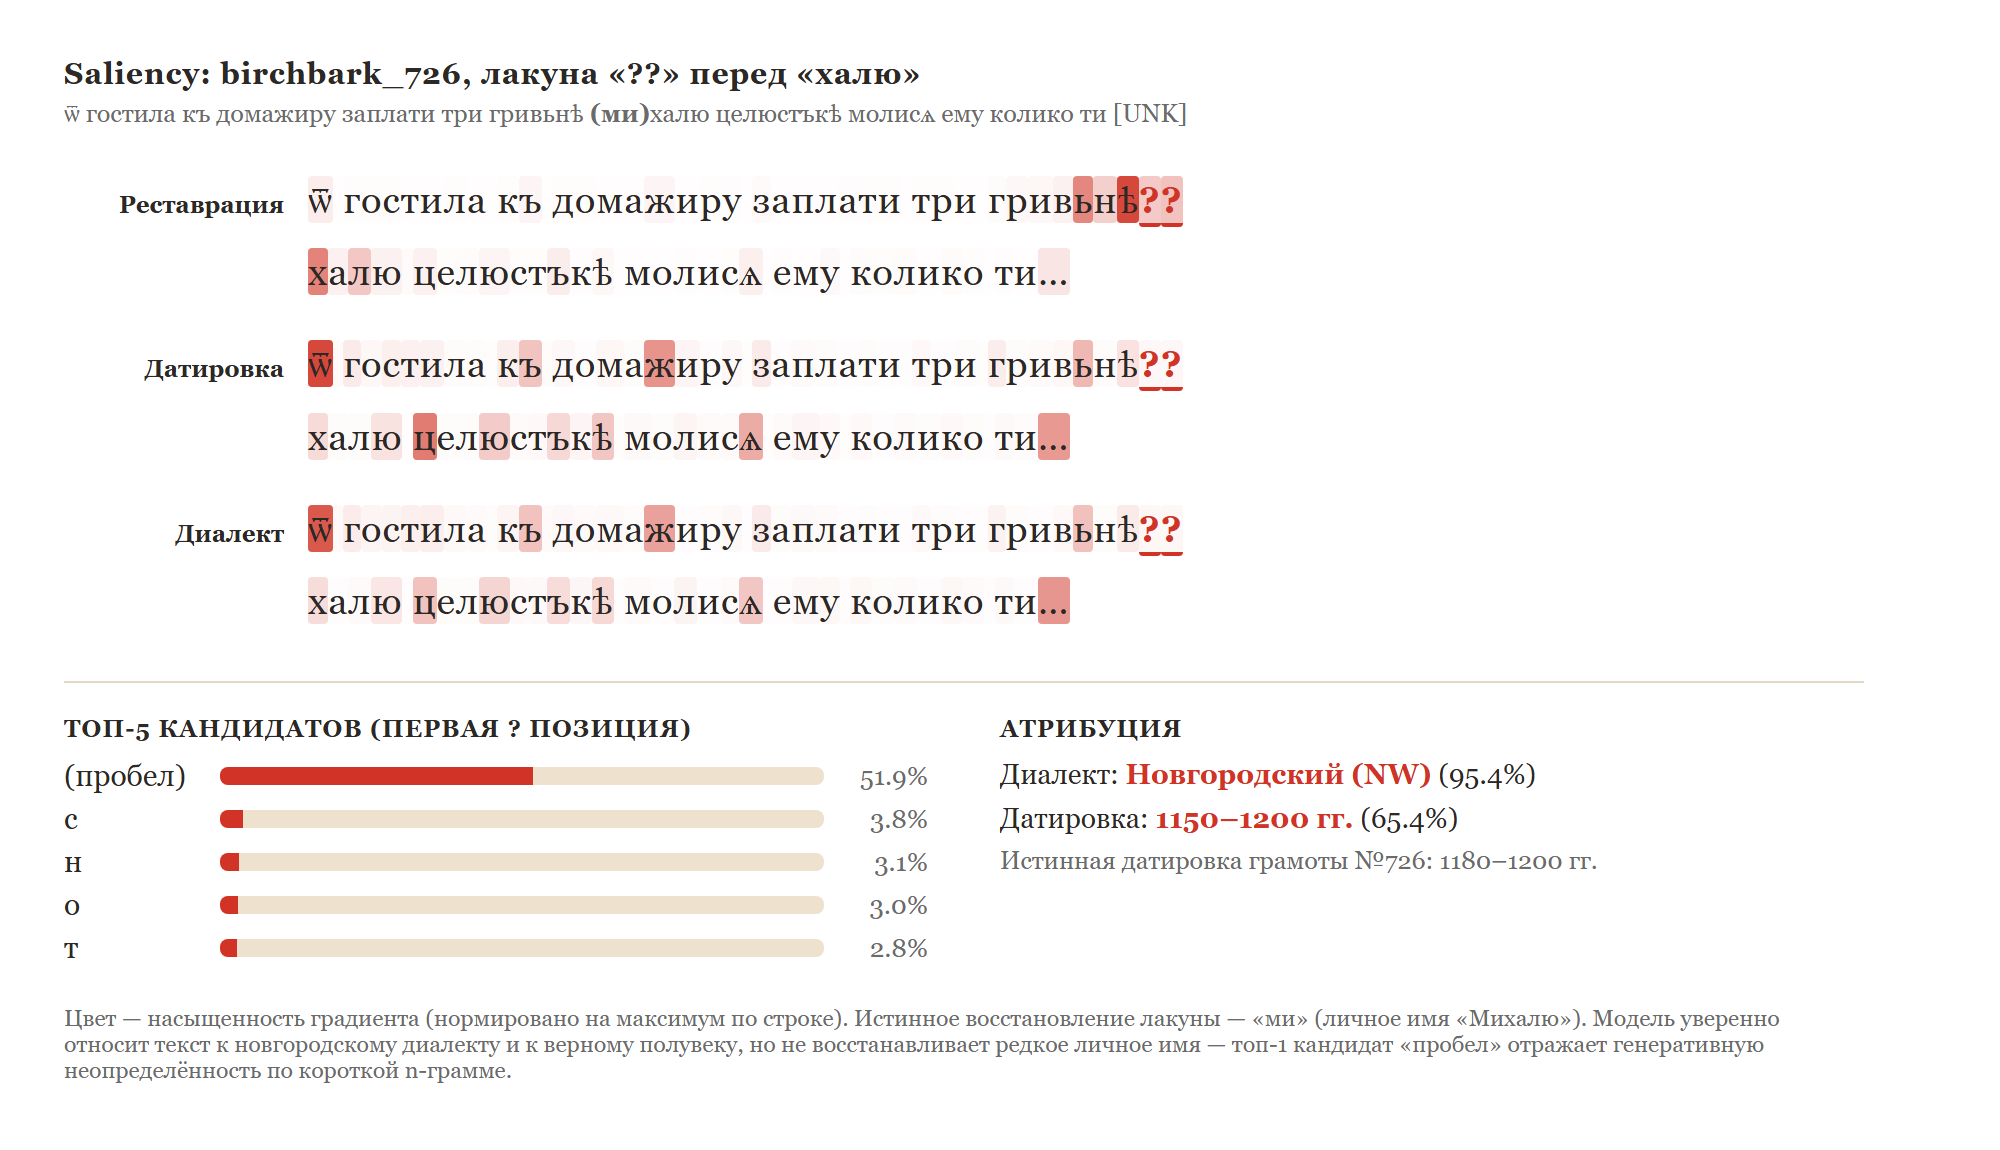
\includegraphics[width=0.95\linewidth]{figures/saliency_diagram.png}
\caption{Gradient saliency for the restoration, date, and dialect heads on a held-out test example (birchbark\_726, a Novgorod letter dated 1180--1200). The masked span (two \texttt{[-]} positions) precedes the personal name \emph{Михалю}; the model correctly attributes the dialect (95.4\%) and half-century (65.4\%) from context alone, but its top restoration candidate for the masked name is a space, reflecting genuine uncertainty over a rare proper noun from a two-character context.}
\label{fig:saliency}
\end{figure}

\begin{figure}[H]
\centering
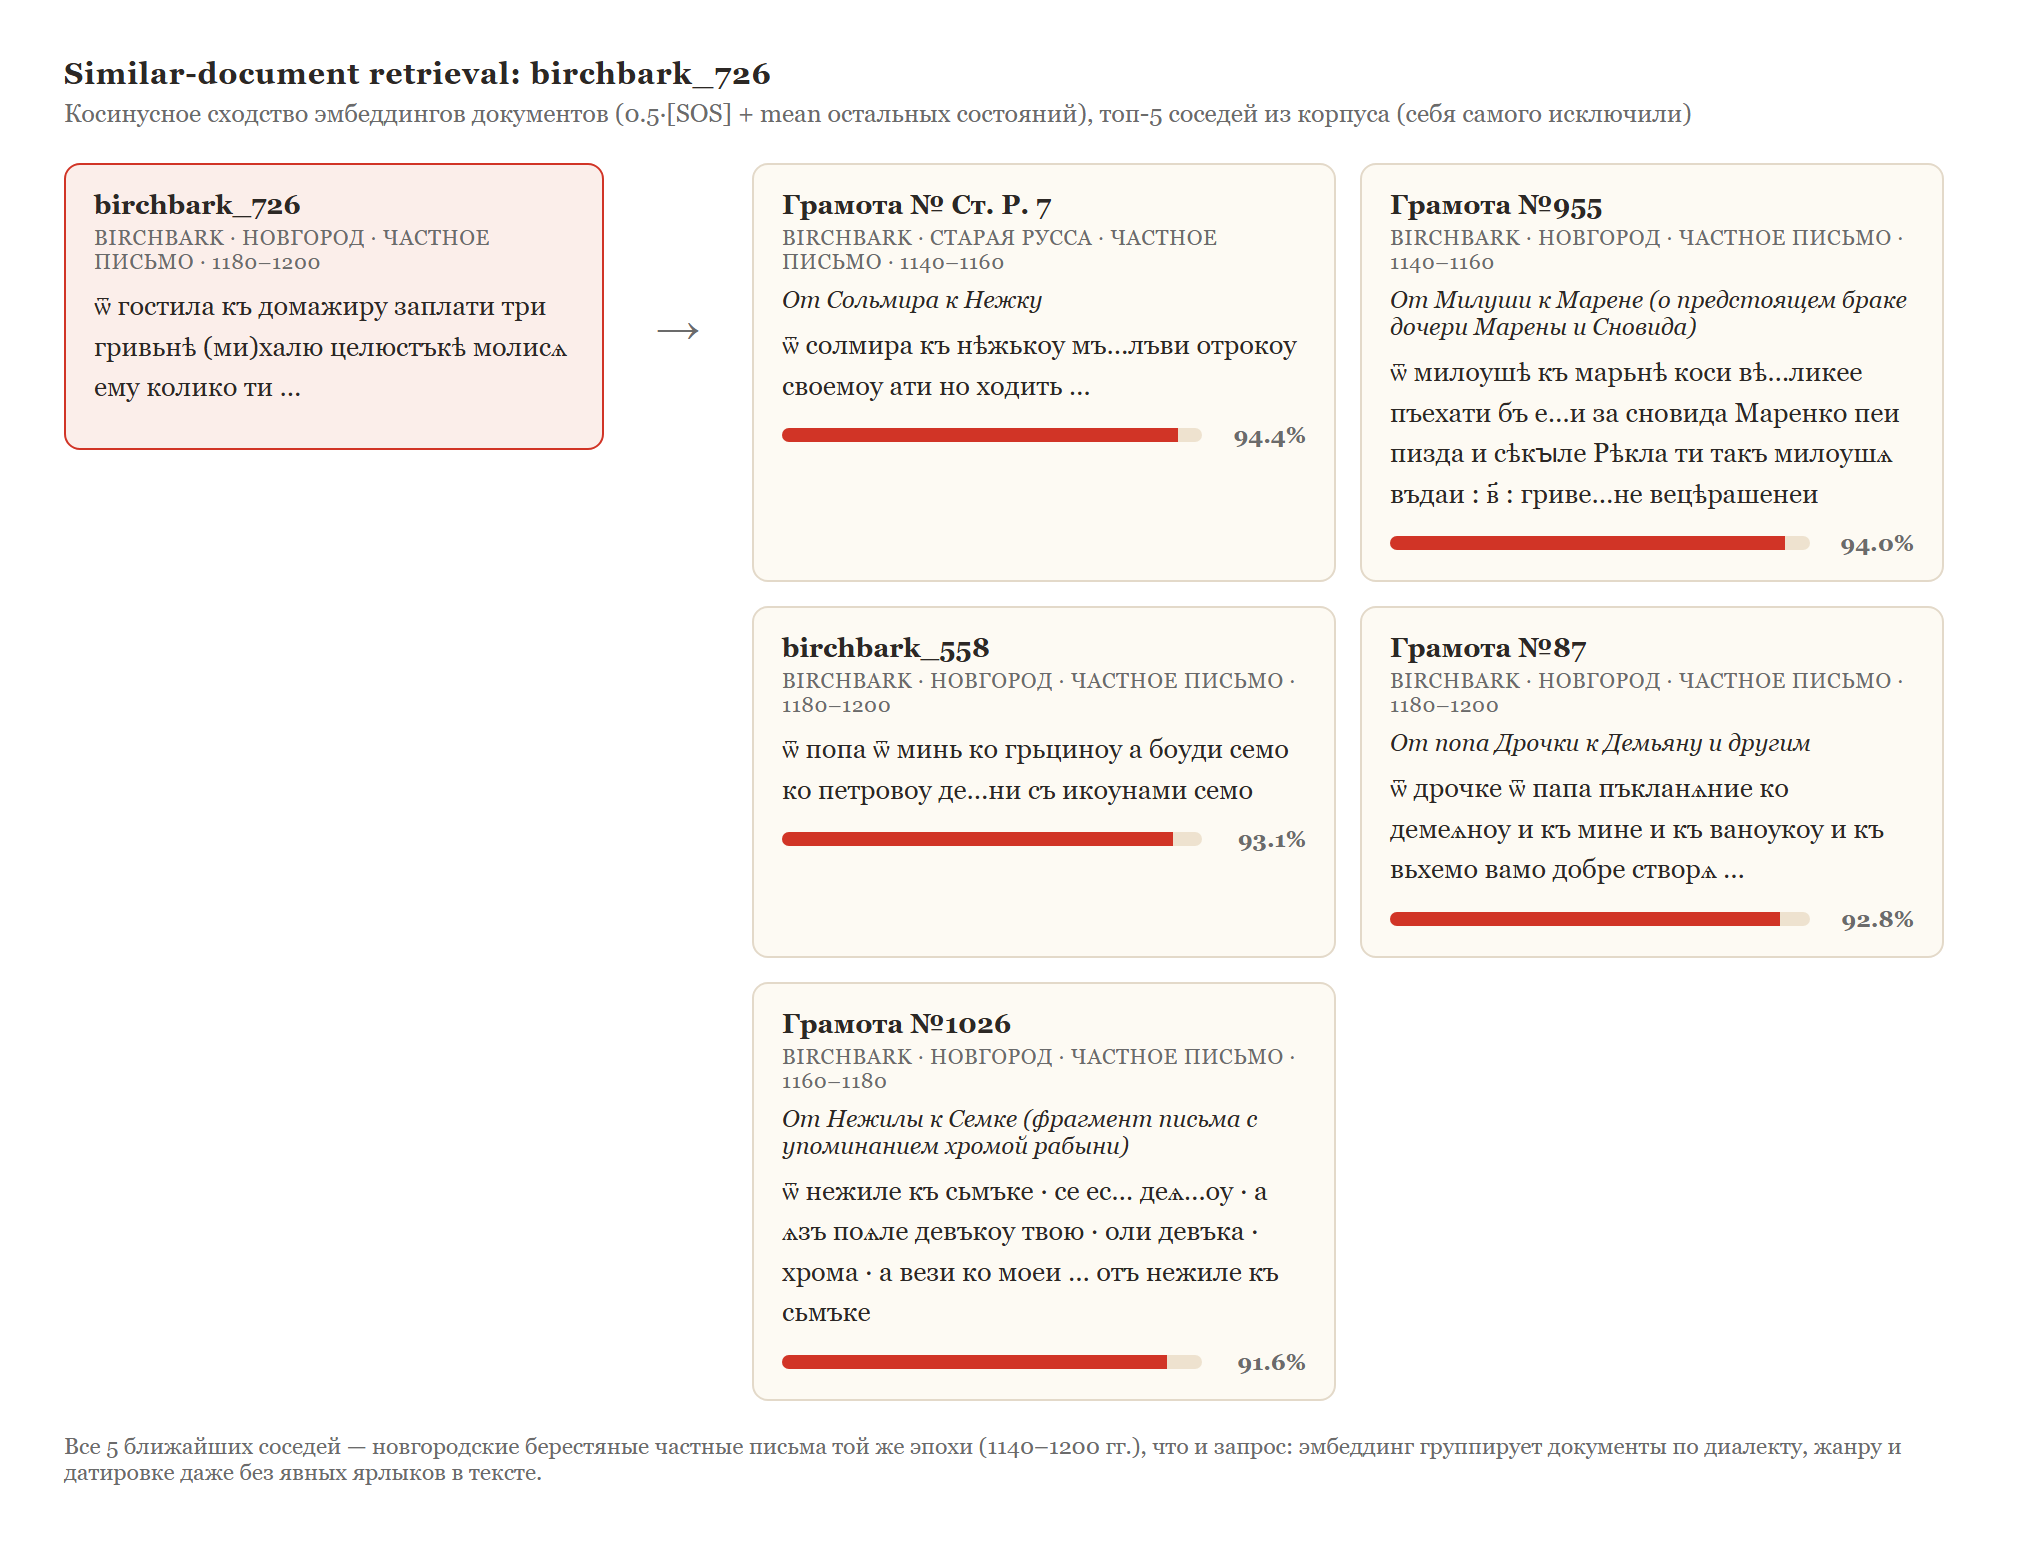
\includegraphics[width=0.95\linewidth]{figures/retrieval_diagram.png}
\caption{Top-5 nearest neighbors by retrieval-embedding cosine similarity for query document birchbark\_726 (excluding the query itself). All five neighbors are Novgorod private letters from the same 1140--1200 window as the query, despite no explicit dialect or date label being visible in the text -- the embedding recovers dialect, genre, and date proximity from form and content alone.}
\label{fig:retrieval}
\end{figure}

\section{Results}

Table~\ref{tab:testab} describes character-level restoration accuracy in the Test A and Test B splits described in Section~\ref{sec:Data}. Top-$k$ accuracy is the proportion of symbol positions that are masked or contain gaps, for which the ground truth character is among  the model’s $k$ best predictions. Test B, based on real-world editorial reconstructions rather than synthetic masking, is consistently more challenging than Test A in all three top-$k$ accuracy metrics, confirming the gap in practical value that the two-stage evaluation described in section~\ref{sec:Data} is designed to reveal. In Test A, the decision to `stop' or `extend' at each step, made by the gap-extension head, is correct 90.0\% of the time, proving that determining \emph{where} a gap ends is comparatively reliable, while restoring \emph{what} was in it remains the harder sub-problem. This picture reverses sharply on Test B (methodology and discussion below): step accuracy there drops to 47.0\% (macro F1 32.0\%), below what a trivial always-predict-the-majority-class baseline would achieve, revealing a real train/deployment distribution mismatch rather than a weaker version of the same skill.

\begin{table}[H]
\centering
\begin{tabular}{|l|r|r|}
\hline
Metric & Test A & Test B \\
\hline
Top-1 accuracy & 18.8\% & 13.8\% \\
Top-3 accuracy & 36.1\% & 32.2\% \\
Top-5 accuracy & 47.8\% & 45.3\% \\
CER (revealed length) & 81.7\% & 87.0\% \\
CER (compress\_unk) & 352.4\% & 883.8\% \\
Region (dialect) accuracy & 91.5\% & 91.3\% \\
Region macro F1 & 89.0\% & 45.4\% \\
Date MAE (years) & 73.3 & 67.3 \\
Gap-expansion (unk) step accuracy & 90.0\% & 47.0\% \\
Gap-expansion macro F1 & 47.4\% & 32.0\% \\
\hline
\end{tabular}
\caption{Metrics on the Test A and Test B splits.}
\label{tab:testab}
\end{table}

Unlike the top-$k$ metrics above, the CER rows score whole-lacuna reconstruction rather than single character positions. For every contiguous masked run (a lacuna) $i$ in Test B, the model's actual iterative decoder produces a predicted string $\mathrm{pred}_i$, compared against the true string $\mathrm{target}_i$ (of length $\mathrm{len}_i$) via the Levenshtein edit distance $d(\cdot,\cdot)$. Every other lacuna in the same example is filled with its ground truth while lacuna $i$ is being scored, so that one lacuna's error cannot cascade into another's. Over the $N$ lacunae in the split, CER is reported as a single micro-average -- summing edit distances and lengths separately before dividing once, rather than averaging each lacuna's own ratio:
\[
\mathrm{CER} = \frac{\sum_{i=1}^{N} d(\mathrm{pred}_i, \mathrm{target}_i)}{\sum_{i=1}^{N} \mathrm{len}_i}.
\]
Because of this micro-averaging, a handful of badly mis-sized lacunae, whose predicted string is far longer or shorter than the truth, can dominate the sum and push CER well above what a per-lacuna average would suggest. Two conditions are reported: with the lacuna's true length revealed ($\mathrm{len}_i$ individual \texttt{[-]} marks, so only the content must be predicted) and with the length hidden (\texttt{compress\_unk}: the lacuna collapsed into a single \texttt{[\#]} marker, so the gap-expansion head must also determine the length itself before restoration can proceed).

Test A's masking is redrawn on the fly during training, so scoring it against the same whole-lacuna harness first requires materializing one fixed set of lacunae to decode against. We reuse the deterministic eval-mode masking already underlying Test A's other reported metrics -- \texttt{KyivanPhysicalCollatorV2(mode="valid")} seeds each document's mask from a hash of its own tokens together with the training seed (42), so the same document always receives the same mask across runs -- with the collator's independent compressed-gap draw (edge tears and geometric-length \texttt{[\#]} gaps, unrelated to the one span being scored) disabled, so each materialized example contains exactly one lacuna of revealed length and nothing else competing for the decoder's attention.

Test B's real editorial reconstructions, by contrast, always come from the source edition with an exact restored length already known (Section~\ref{sec:Data}), so the pre-built dataset never contains a genuine unknown-length \texttt{[\#]} case on its own. To still evaluate the gap-expansion head against real damage, we recast each of Test B's 1{,}721 real lacunae as a single \texttt{[\#]} marker and score the head's one-shot stop/extend decision against the true label collator\_v2.py itself uses when constructing a compressed gap during training (\texttt{multi} iff the lacuna is longer than one character), isolating one lacuna at a time exactly as the CER evaluation above does.

This is where the sharpest finding in this evaluation appears. Real damage in Test B is dominated by single-character lacunae (912 of 1{,}721, 53.0\%) -- more common than multi-character gaps, if only barely. The gap-expansion head, however, predicts \texttt{multi} for every single one of the 1{,}721 lacunae we tested, without exception. This is not random noise: during training, a compressed gap's length is drawn as $\mathrm{geometric}(p{=}0.25) - 1$, conditioned on being non-empty, which puts roughly 75\% of the head's training signal on multi-character gaps; edge-tear damage (10\% of training documents) is multi-character by construction (2--20 chars). The head has, in effect, learned the training-time class prior rather than a genuine content-dependent stopping rule, and a real corpus with a near-even (53/47) split exposes this: 47.0\% step accuracy is \emph{worse} than the 53.0\% a trivial always-\texttt{single} baseline would score on this same data. Test A's own reported gap-expansion numbers already hint at the same issue from the other side -- 90.0\% step accuracy against only 47.4\% macro F1 is itself the signature of a majority-class collapse, just against Test A's own (multi-skewed) synthetic mask distribution rather than Test B's real one. Recalibrating the training-time gap-length distribution to match Test B's true length distribution, rather than an assumed geometric prior, is a direct, low-effort follow-up.

The \texttt{compress\_unk} condition illustrates this micro-averaging effect concretely: forcing the model to also discover a lacuna's length from a single \texttt{[\#]} marker pushes overall CER to 883.8\% on Test B (352.4\% on Test A, same materialized examples as the revealed-length condition above), driven almost entirely by the shortest lacunae in each split ($\mathrm{CER}=1975.7\%$ at length 1 on Test B, $1964.7\%$ on Test A) -- with no length cue, the gap-expansion head has no strong signal to stop after one character, and a several-character overshoot on a length-1 target already multiplies the local error many times over. This is the same always-\texttt{multi} bias documented above: with no length revealed, the head defaults to expanding, which is precisely wrong on the majority of real lacunae. CER falls into the 260--370\% range once the true length reaches 6 characters or more on both splits, where a similar absolute overshoot is a proportionally smaller error.

\section{Conclusion}

We presented Kyivan, a character-level bidirectional encoder with rotary positional embeddings that jointly restores missing text, determines the length of gaps of unknown extent, and attributes a document's dialect and approximate date, adapting the Ithaca/Aeneas line of work \cite{assael2022,assael2025} to Old East Slavic material for the first time. The corpus this model is trained on is deliberately curated around \emph{grammoty} -- birch-bark letters and chancellery/business documents -- rather than epigraphy: even after accounting for source imbalance, restoration on Test B (real editorial reconstructions, dominated by birch-bark and epigraphic lacunae) reached 13.8\% top-1 / 45.3\% top-5 character accuracy. The auxiliary tasks are a mixed picture: dialect attribution is genuinely reliable (91.3\% accuracy on Test B), but gap-expansion is not -- 90.0\% step accuracy on Test A's synthetic masks conceals a majority-class collapse that a near-evenly-split real corpus exposes outright, with Test B step accuracy (47.0\%) falling below what always predicting the majority class would already achieve.

These numbers sit well below Ithaca/Aeneas's own reported figures, and we do not read that gap as a shortcoming of the architecture. Our training corpus is roughly two orders of magnitude smaller than the Greek epigraphic corpus Ithaca and Aeneas draw on, and it is far less formulaic: birch-bark letters and chancellery acts are individually composed correspondence and administrative prose, not the templated decrees and dedications that make Greek epigraphic restoration comparatively tractable. We therefore present Kyivan's numbers as a first benchmark for Old East Slavic restoration on real, heterogeneous manuscript material, not as a direct comparison against a task with a fundamentally different data regime. A concrete methodological lesson from this work, worth stating for anyone building a similar pipeline, is that an earlier version of our own evaluation split documents into overlapping fixed-length windows before the train/test split was drawn, letting near-duplicate windows of the same document land on both sides of the split; the resulting leakage inflated every reported metric substantially before it was identified and fixed by switching to one row per document with dynamic, random-length crops drawn per epoch.

Several directions remain open. The most immediately actionable is recalibrating the gap-expansion head's training-time length distribution: it currently predicts \texttt{multi} unconditionally, having learned the geometric prior it was trained under (roughly 75\% multi-character) rather than a real stopping rule, and Test B shows the true distribution of physical damage is close to even (53\% single-character). The broader, more promising lever beyond that is data, not architecture: our own params-to-corpus-size accounting suggests the current model is already close to appropriately sized for $\sim$4,400 training documents, so a wider hidden dimension is unlikely to help without more data, whereas the Novgorod/Pskov charter sub-collection within our corpus is itself under-sampled (15 documents) relative to what has actually been published and could be extended. Feeding a document's own predicted dialect and date back into the restoration head as an explicit conditioning signal is architecturally straightforward but requires care to avoid a train/inference mismatch, since ground-truth labels are available only at training time; a self-conditioning scheme using the model's own first-pass predictions is the safer route. Finally, the saliency-map and retrieval-based case studies outlined in Section~\ref{sec:Data} (Figures~\ref{fig:saliency}, \ref{fig:retrieval}) remain to be filled in with qualitative examples from the trained checkpoint, which would let historians inspect concretely which characters and parallel documents drive a given restoration.

% ════════════════════════════════════════════════════════════════════════════
% REFERENCES
% ════════════════════════════════════════════════════════════════════════════
\printbibliography[title={References}]

\end{document}
